\section{Systeme mit mehreren Taktraten}
%\subsection{Taktraten�nderung}

\vspace{-0.5cm}

\begin{minipage}{11.5cm}
	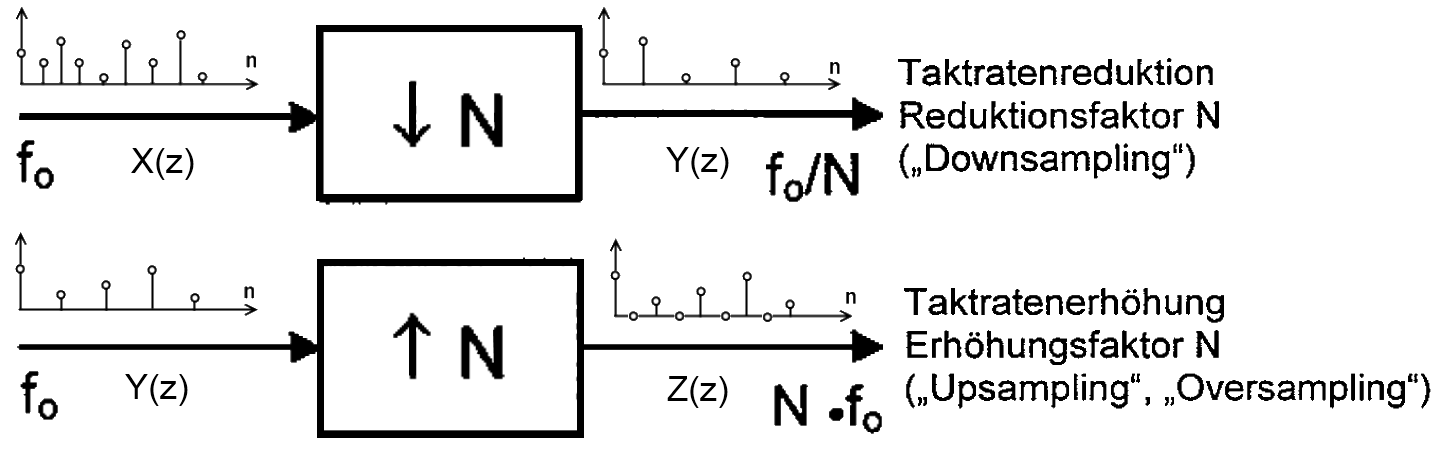
\includegraphics[width=12cm]{Content/VerschTaktraten/UpDownSampling.png}
\end{minipage}
\begin{minipage}{7cm}	
	\begin{itemize}
		\item Mittels Downsampling kann unn�tig hoher Rechenaufwand vermieden werden.
		\item Spektrale Verschiebungen sind m�glich um Anpassungen zwischen verschiedenen Normen durchzuf�hren
		\item Bei der AD- oder DA-Wandlung kann der Analogaufwand vermindet werden.
	\end{itemize}
\end{minipage}

%\vspace{0.1cm}

\begin{minipage}[t]{0.5\textwidth}
\subsection{Dezimierung/Downsampling Beispiel}
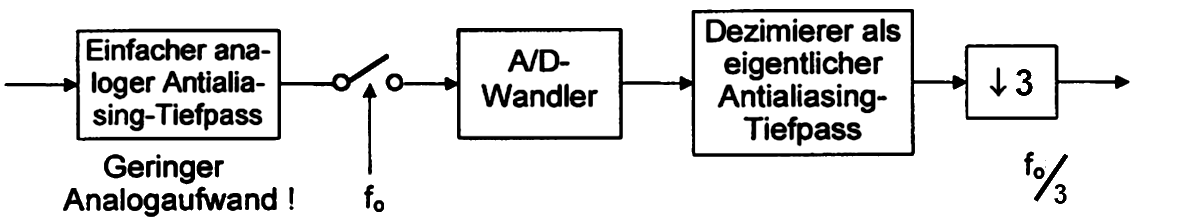
\includegraphics[width=\textwidth,trim= 0cm 0cm 0cm 0.25cm]{Content/VerschTaktraten/DownSampPrinzip.png}\\
%Farbig
%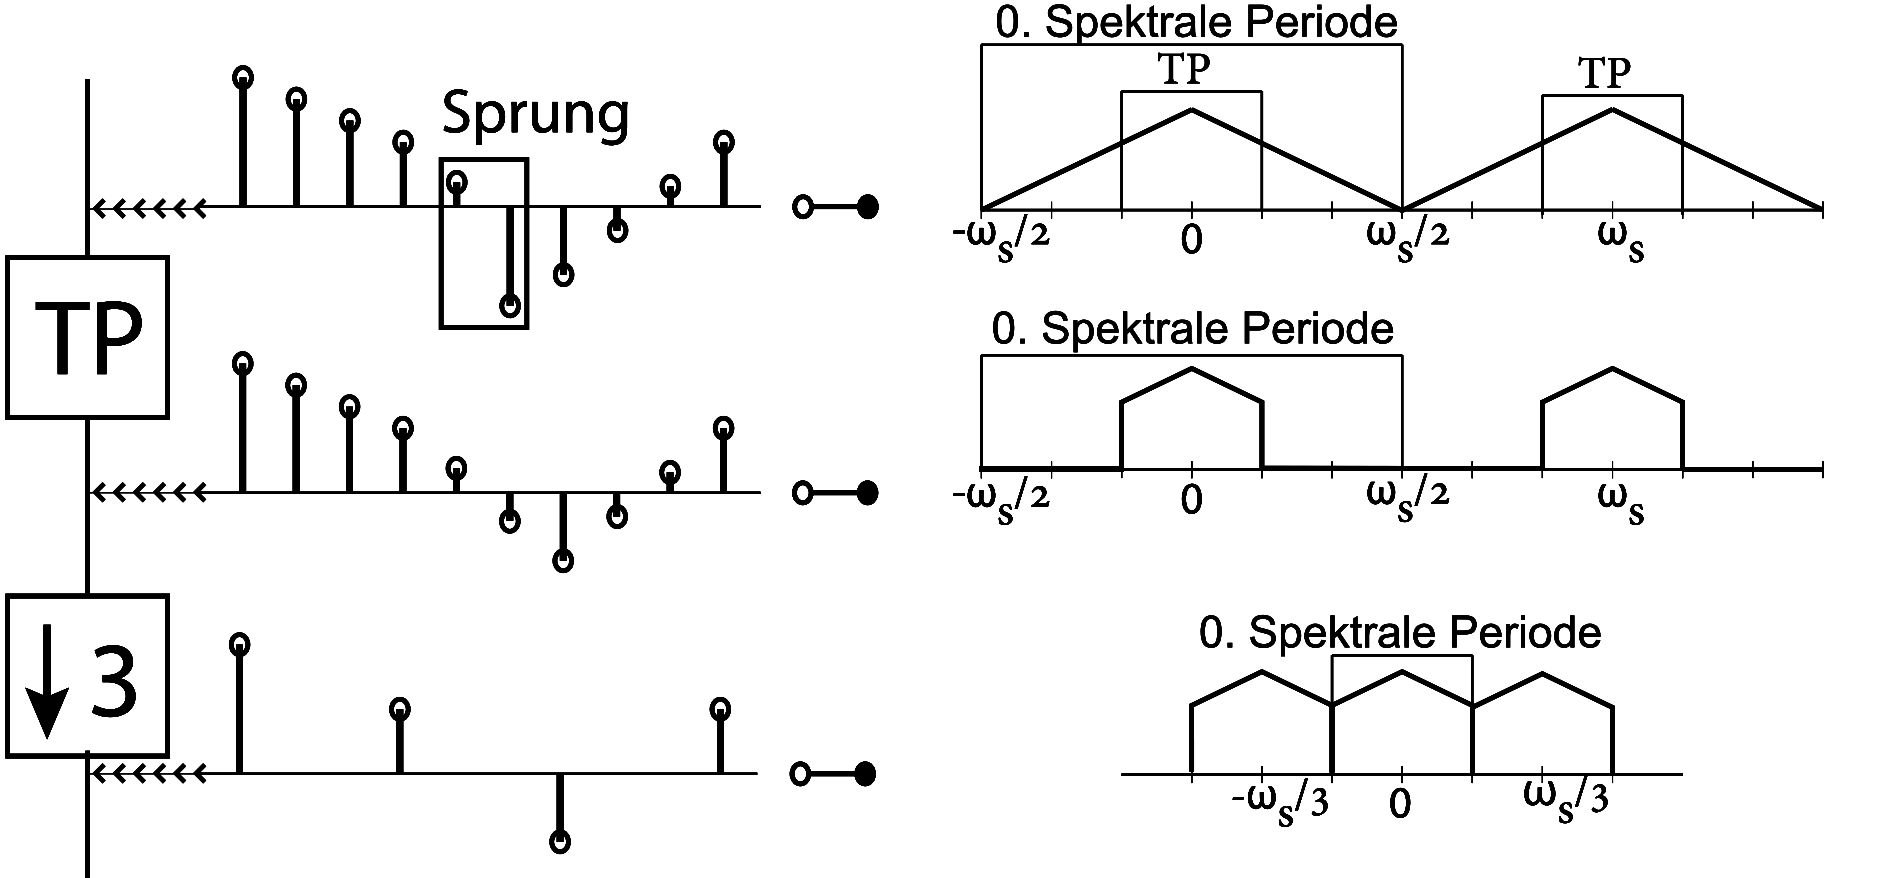
\includegraphics[width=\textwidth,trim= 0cm 0cm 0cm 0cm]{Content/VerschTaktraten/downsampling.pdf}
%Schwarzweiss
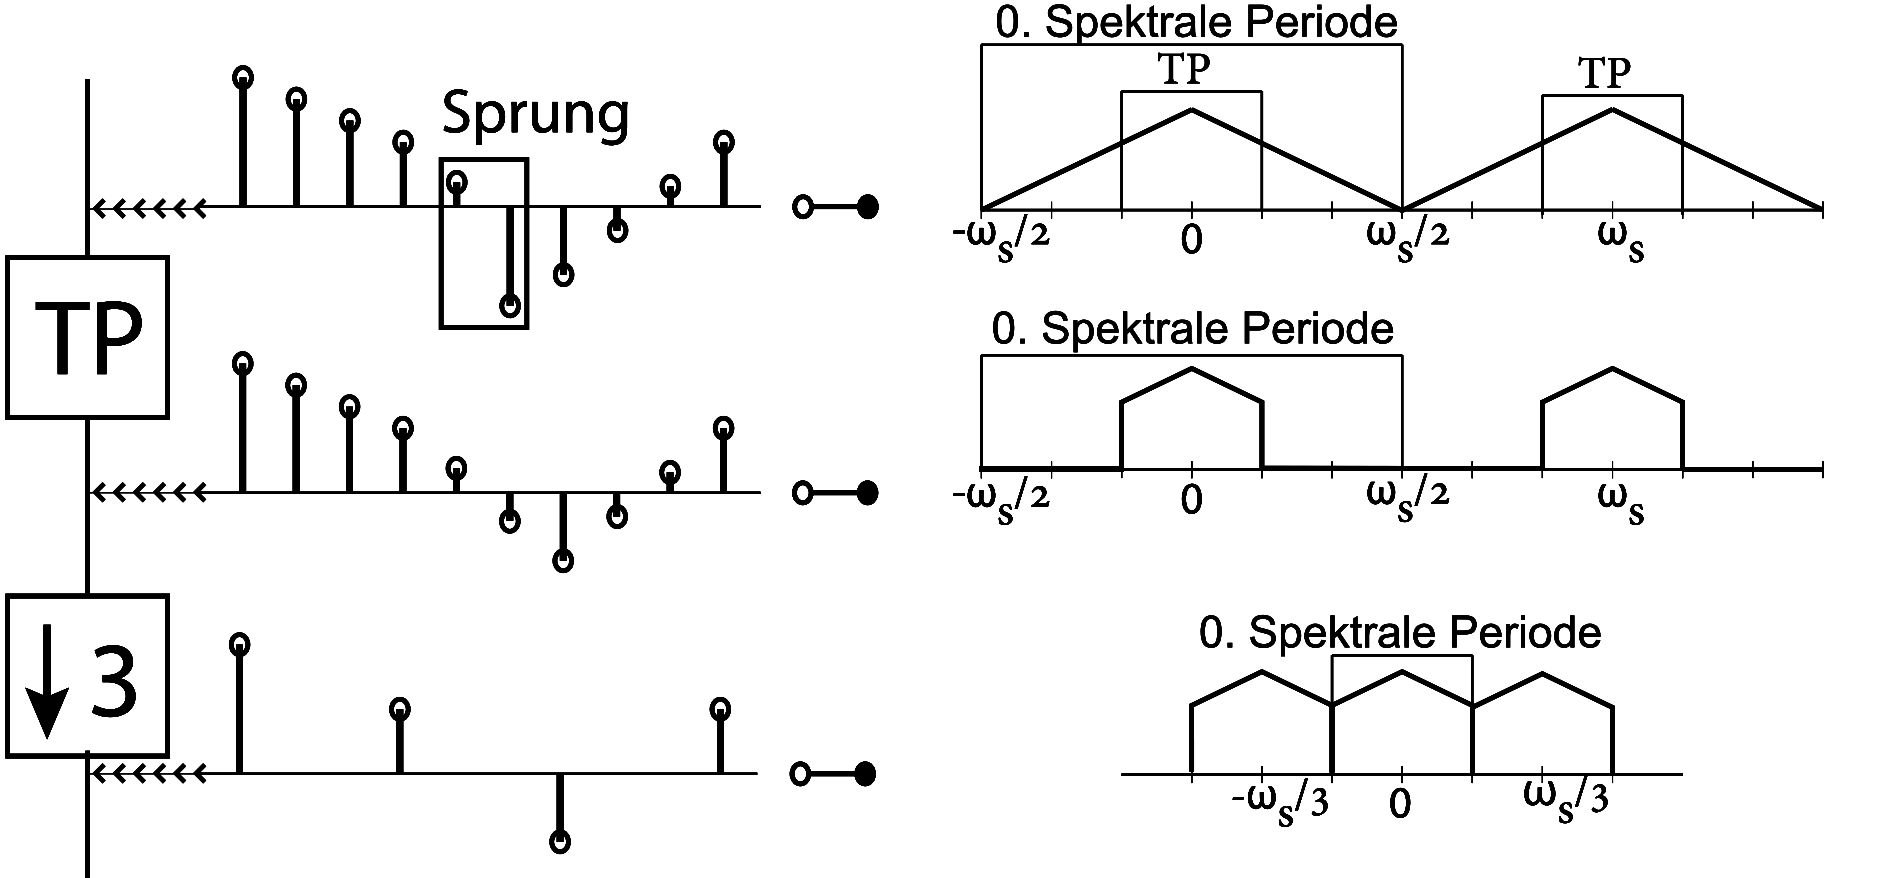
\includegraphics[width=\textwidth,trim= 0cm 0cm 0cm 0cm]{Content/VerschTaktraten/downsampling.png}
\end{minipage}
\begin{minipage}[t]{0.5\textwidth}
\subsection{Interpolation/Upsampling Beispiel}
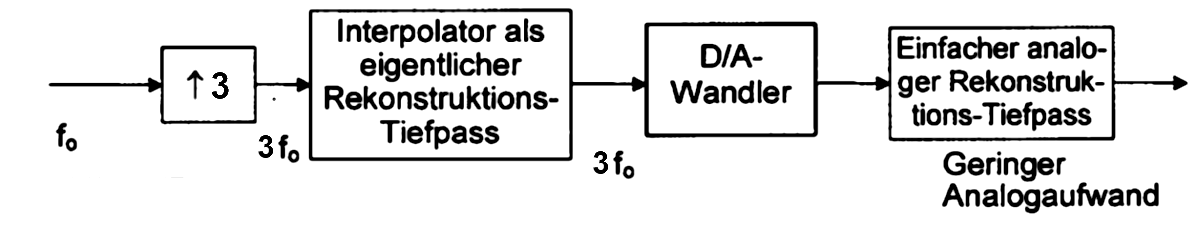
\includegraphics[width=\textwidth,trim= 0cm 0.25cm 0cm 0.25cm]{Content/VerschTaktraten/UpSampPrinzip.png}\\
%Farbig
%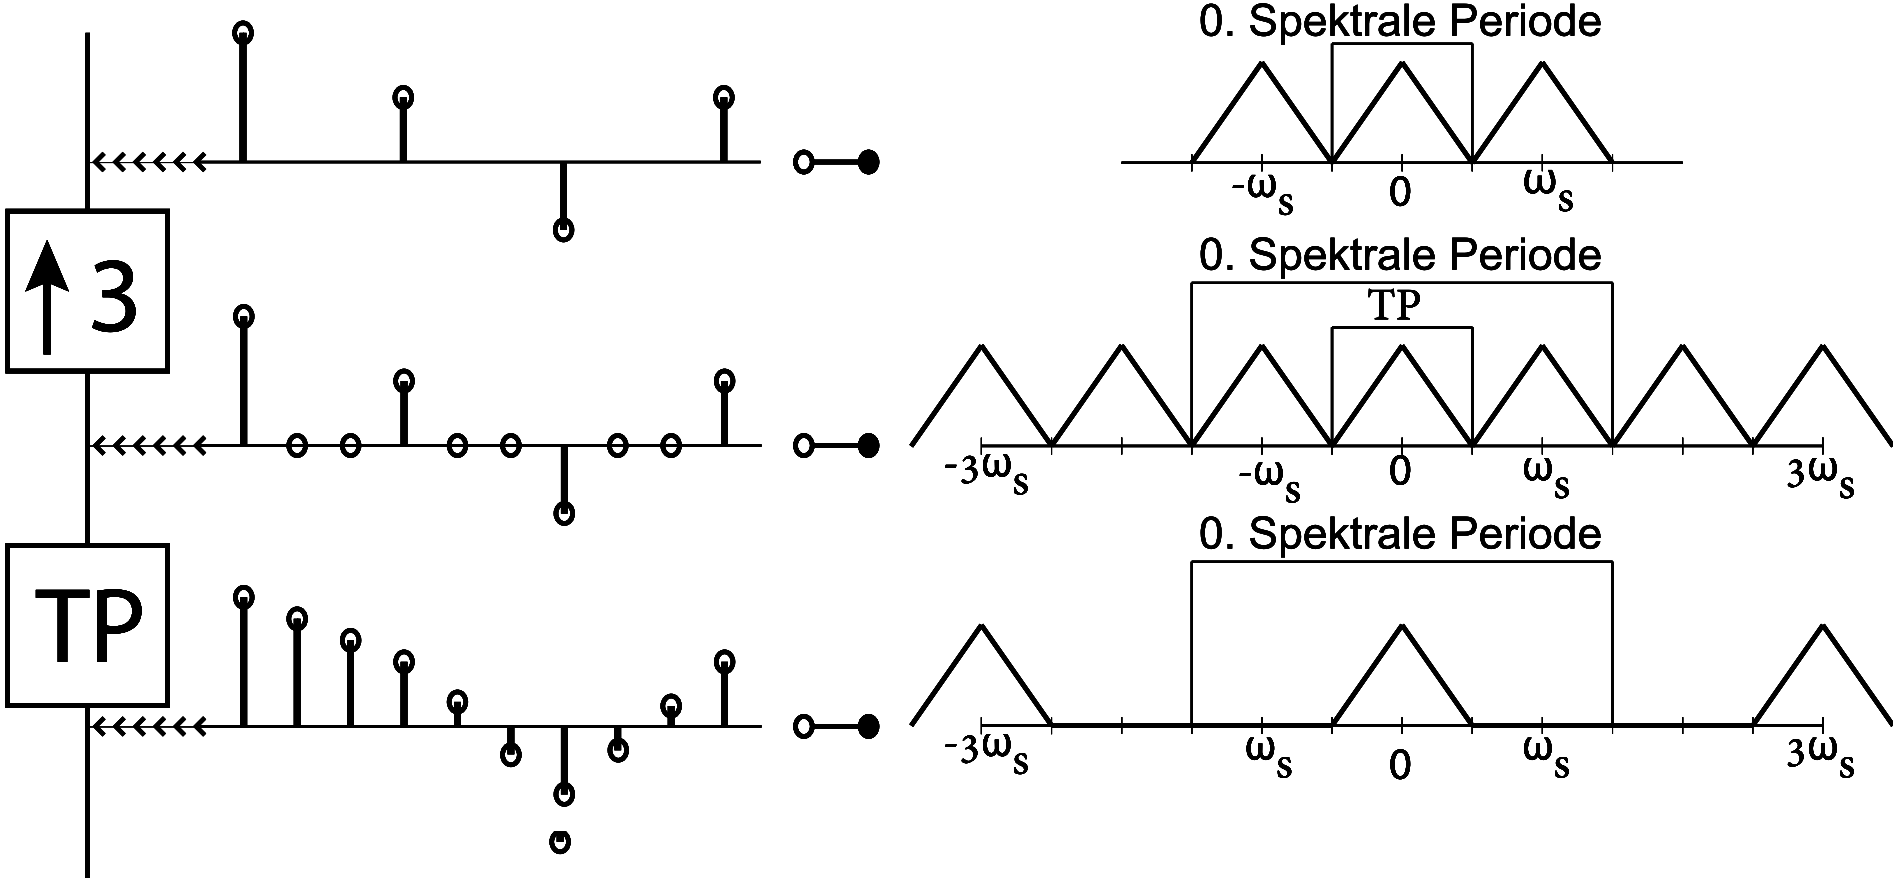
\includegraphics[width=\textwidth,trim= 0cm 0cm 0cm 0cm]{Content/VerschTaktraten/upsampling.pdf}
%Schwarzweiss
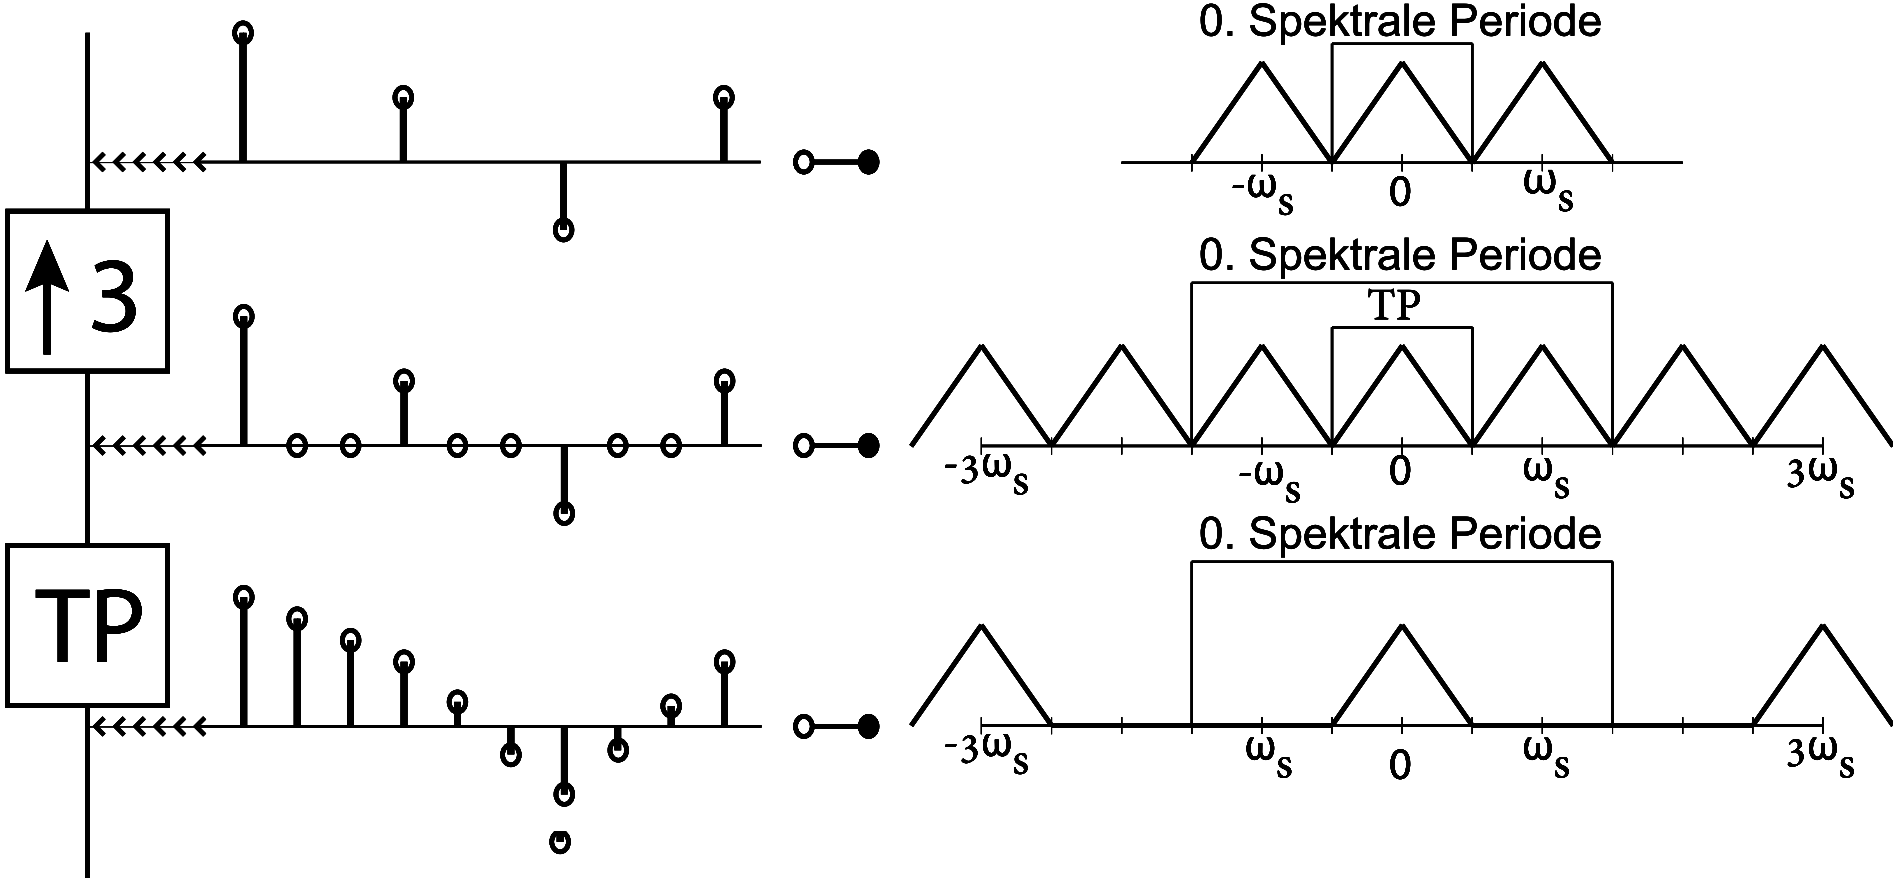
\includegraphics[width=\textwidth,trim= 0cm 0cm 0cm 0cm]{Content/VerschTaktraten/upsampling.png}
\end{minipage}
%\footnotesize 
\textbf{Oversampling:} Falls Dezimierer mit feinerer Quantisierung gerechnet wird: $\rightarrow$ $SNR=K+6.02 \cdot n + 10\cdot \log(OSR)$\\
\textbf{Normierte Frequenzen:} Wenn man mit normierten Frequenzen rechnet, normiert man die Abtastfrequenz $f_s$ auf $2\pi$. Dazu wird jeweils die Frequenzachse gestreckt oder gestaucht, bis die Abtastfrequenz auf $2\pi$ zu liegen kommt.\\
\normalsize
$\frac{N_{oe4}}{2}=\frac{P_{e4}}{OSR\cdot f_0}=\frac{q^2}{12\cdot OSR \cdot f_0}$ \qquad $P_{e4}=\frac{q^2}{12}$ \qquad Ist nur hoeher als normal wenn Dezimierer mit feinerer Quantisierung.
                                              


%\begin{minipage}[t]{0.36\textwidth}
	%\begin{tabular}{ll}
		%Maximale Signalfrequenz&$f_{max}$\\
		%Minimale Abtastfrequenz& $f_0=2\cdot f_{max}$\\
		%�berabtastungsfaktor& $OSR=\frac{f_s}{2\cdot f_{max}}$\\
		%Abtastfrequenz&$f_s=OSR\cdot f_0$\\
		%Aufl�sung&$n$\\
	%\end{tabular}
%\end{minipage}
%\begin{minipage}[t]{0.64\textwidth}
%
%\end{minipage}
%
%\begin{tabular}{p{4.5cm}p{2.5cm}p{2.5cm}p{6cm}}
%Abtastungsart&Rauschleistung&Leistungsdichte&SNR\\
%Normal&$P_e=\frac{q^2}{12}$&$N_{oe}=\frac{q^2}{12\cdot f_0}$&$SNR=K+6.02\cdot n$\\
%�berabgetastet 1)&$P_e=\frac{q^2}{12*OSR}$&$N_{oe}=\frac{q^2}{12\cdot f_0}$&$SNR=K+6.02 \cdot n + 10\cdot \log(OSR)$\\
%%Noise Shaping 1.Ord&&&\\
%%Noise Shaping 2.Ord&&&\\
%\end{tabular}

\vspace{-0.6cm}

\subsection{Noise-Shaping}

\vspace{-0.5cm}

\begin{minipage}{10cm}
Ein Noise-Shaper unterdr�ckt das Quantisierungsrauschen im Frequenzbereich des
Nutzbandes und verst�rkt es im Bereich daneben. Man kann also das Rauschen in Frequenzbereiche schieben, welche sowieso abgeschnitten werden.
\end{minipage}
\vspace{0.1cm}
\begin{minipage}{9cm}
	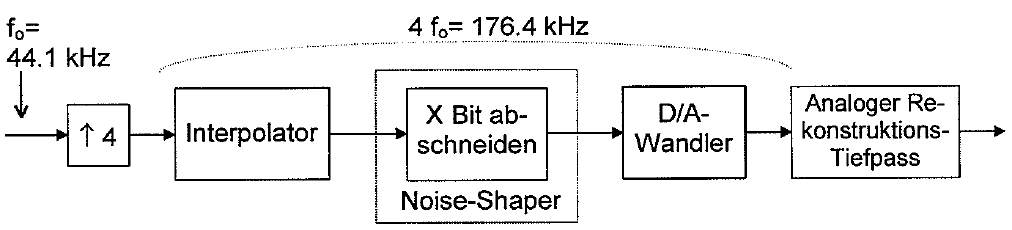
\includegraphics[width=9cm]{Content/VerschTaktraten/Noise-Shaping_1.PNG}
\end{minipage}\\
\begin{minipage}[t]{7cm}
	\textbf{Noise-Shaper erster Ordnung}\\
	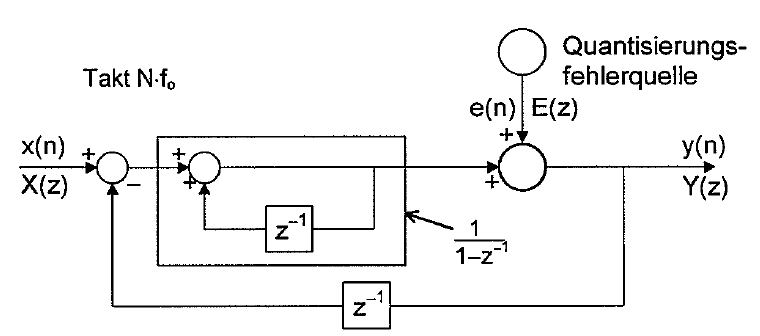
\includegraphics[width=7cm]{Content/VerschTaktraten/Noise-Shaping_2.PNG}
\end{minipage}
\begin{minipage}[t]{6cm}
	\textbf{Noise-Shaper zweiter Ordnung}\\
	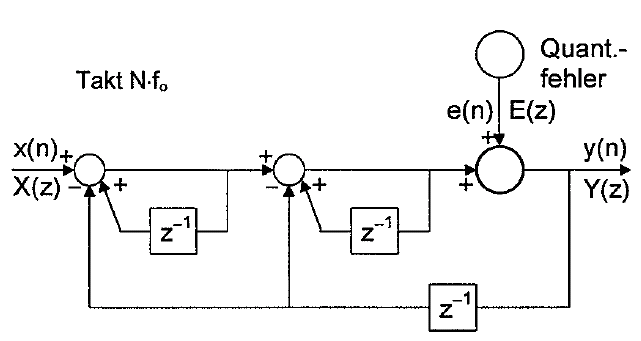
\includegraphics[width=6cm]{Content/VerschTaktraten/Noise-Shaping_3.PNG}
\end{minipage}
\begin{minipage}[t]{6cm}
	Rauschleistung: $P_{eN} = k_n \frac{q_e^2}{12}$ \\ \\
    $Y_{1st}(z) = X(z) + E(z)(1-z^{-1})$\\ 
    $k_{1st} = \frac{2}{N} \left[ 1 - \frac{N}{\pi} \sin{(\frac{\pi}{N})}\right] \approx \frac{\pi^2}{3 N^3}$
    \\
	
	$Y_{2nd}(z) = X(z) + E(z)(1-z^{-1})^2$ \\	
    $k_{2nd} \approx \frac{\pi^4}{5 N^5}$\\
		$N$: �berabtastungsfaktor (OSR)
		
	
\end{minipage}

\subsection{Oversampling $\Delta\Sigma$-DA und -AD-Wandler}
\begin{minipage}[t]{12cm}
	\textbf{DA-Wandler}\\
	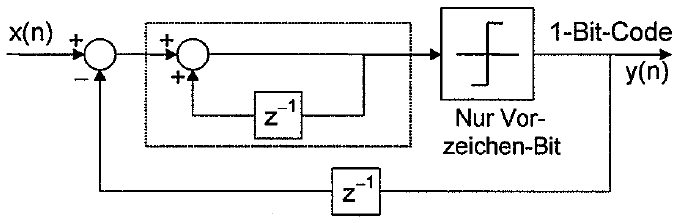
\includegraphics[width=6cm]{Content/VerschTaktraten/Delta_Sigma_1.PNG}
	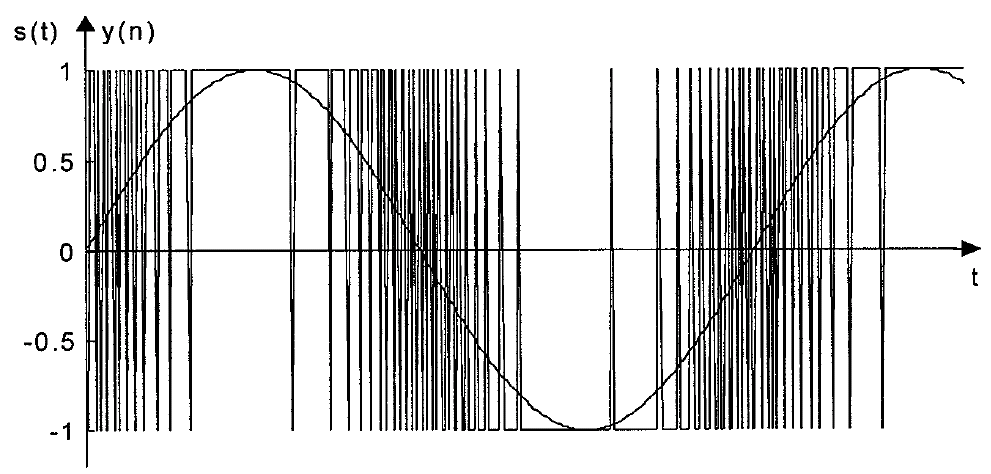
\includegraphics[width=6cm]{Content/VerschTaktraten/Delta_Sigma_2.PNG}
	Durch den Noise-Shaping Block und mit sehr hohem Oversampling\\
	(N=128,256) kann der DA-Wandler mit nur einem Bit Aufl�sung\\
	auskommen, bei gleichbleibender SNR.
\end{minipage}
\begin{minipage}[t]{6cm}
	\textbf{AD-Wandler}\\
	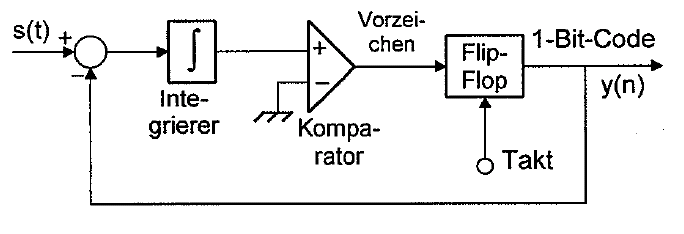
\includegraphics[width=6cm]{Content/VerschTaktraten/Delta_Sigma_3.PNG}
	Durch eine hohe Taktfrequenz des Flip Flops wird ein bin�res Signal erzeugt,
	welches nach einer Dezimierung und einem Downsampling verwendetet werden kann.
\end{minipage}